% This template was created by Stephen V. Cole
% for Benedictine College CS398 S14 
% with help from template created by Brian R. Hall
% Assistant Professor, Champlain College
% www.brianrhall.net
% and Title Page template (see below)

% % % % % 
% Document format info
% % % % %
\documentclass[12pt]{article}
\usepackage[margin=1in]{geometry}
\usepackage[pdftex]{graphicx}
\usepackage{url}
\usepackage{amsmath}
\pagestyle{plain}
\setlength\parindent{0pt}

% 1.5-space doc
\baselineskip18pt

% % % % %
% Custom commands/macros
% % % % %

% Format for tilde character `~' ; to insert this character, just type \mytilde
\newcommand{\mytilde}{\raise.17ex\hbox{$\scriptstyle\sim$}}

% Example macro: as a result of this definition, you can type `\openssl' anywhere in the document
%     to produce the string `openssl' in typewriter-style font (think Courier).
\newcommand{\openssl}{{\tt openssl }}

% TeXstudio: I got tired of typing this out, so I created a macro to save a 
% few keystrokes and a stretch to the `shift' key each time.
\newcommand{\ts}{TeXstudio}

% % % % % % % % % % % % % % % % % % % % % % % % % %
% % Tile page def
%%%%
% Classic Lined Title Page 
% LaTeX Template
% Version 1.0 (27/12/12)
%
% This template has been downloaded from:
% http://www.LaTeXTemplates.com
%
% Original author:
% Peter Wilson (herries.press@earthlink.net)
% Modified by Steve Cole for Benedictine College CS398 S14
% License:
% CC BY-NC-SA 3.0 (http://creativecommons.org/licenses/by-nc-sa/3.0/)
% 
% Instructions for using this template:
% This title page compiles as is. If you wish to include this title page in 
% another document, you will need to copy everything before 
% \begin{document} into the preamble of your document. The title page is
% then included using \titleAT within your document.
%
%%%%

%----------------------------------------------------------------------------------------
%	PACKAGES AND OTHER DOCUMENT CONFIGURATIONS
%----------------------------------------------------------------------------------------

%\documentclass{book}

\usepackage[svgnames]{xcolor} % Required to specify font color

%\newcommand*{\plogo}{\fbox{$\mathcal{PL}$}} % Generic publisher logo

%----------------------------------------------------------------------------------------
%	TITLE PAGE
%----------------------------------------------------------------------------------------

\newcommand*{\titleAT}{\begingroup % Create the command for including the title page in the document
\newlength{\drop} % Command for generating a specific amount of whitespace
\drop=0.1\textheight % Define the command as 10% of the total text height

\rule{\textwidth}{1pt}\par % Thick horizontal line
\vspace{2pt}\vspace{-\baselineskip} % Whitespace between lines
\rule{\textwidth}{0.4pt}\par % Thin horizontal line

\vspace{\drop} % Whitespace between the top lines and title
\centering % Center all text
\textcolor{Red}{ % Red font color
{\Huge Computer Security Semester Project}\\[0.5\baselineskip] % Title line 1
{\Huge WEP Vulnerabilities and Cracking}} % Title line 3

\vspace{0.25\drop} % Whitespace between the title and short horizontal line
\rule{0.3\textwidth}{0.4pt}\par % Short horizontal line under the title
\vspace{\drop} % Whitespace between the thin horizontal line and the author name

% Author names
{\Large \textsc{Byte Me}}\par 
\vspace{12pt}
{\large \textsc{Augustine Calvino}}\par 
\vspace{8pt}
{\large \textsc{Stephen Noffke}}\par 
\vspace{30pt}

\vfill % Whitespace between the author name and footer

% Footer

\includegraphics[height=1.25in]{BC_logo.png} \par
\vspace{5pt}
{\Large \textsc{Benedictine College}}\par
{\large \textsc{CS398b: Computer Security}}\par
{\large \textsc{Spring 2014}}\par

\vspace*{\drop} % Whitespace under  text

\rule{\textwidth}{0.4pt}\par % Thin horizontal line
\vspace{2pt}\vspace{-\baselineskip} % Whitespace between lines
\rule{\textwidth}{1pt}\par % Thick horizontal line

\endgroup}
% % % % % % % % % % % % % % % %

% % % % %
%  Start of actual typesetting code
% % % % %
\begin{document}

% Title page
\thispagestyle{empty}  % Suppress page number printing
\titleAT 
\pagebreak

% Rest of document
\setcounter{page}{1}  	% Reset page number count

% 1st section
\section{Introduction}   
\label{section:intro}
Wi-Fi Systems have notably increased in usage to the point that they are almost ubiquitous in corporate and home settings.  To keep information private and prevent unauthorized access to Wi-Fi networks, the WEP algorithm was created.  However, it fails to meet its desired goals due to inherent flaws in its implementation.  In this project, we will explain the WEP standard in its different components.  Using this knowledge, we will explain the flaws in this system intended for network security, and will demonstrate an attack exploiting them using aircrack-ng.

% 2nd section
\section{Background}
\label{sec:bckgd}
WiFi is integral to our daily lives.  Almost everyone uses it every day, whether in checking emails, bank accounts, social media, the weather, or just browsing news.  This information is all sent through the air in electromagnetic pulses, allowing anyone with the proper hardware (i.e., anyone with a wireless compatible laptop) to intercept them and view the data they represent.  Private information such as that found on banking, government, or university websites is usually encrypted at the application layer using https, but not always.  To keep information private by default, as well as to prevent unauthorized access to Wi-Fi system resources such as bandwidth, standards of link layer encryption consequently were developed.  The first mainstream implementation of such an encryption algorithm was the \textit{Wired Equivalency Privacy} (WEP) standard, created in September 1999.  This standard supposedly would protect users from unauthorized access to their network, but unfortunately it failed to meet its goal.  By 2001, its flaws were well known and commonly exploited, and in 2004 it was officially deprecated by the IEEE.  It was replaced with the quick fix of WAP, which has since been updated to the current norm WPA2.  Nonetheless, between replacement costs, lack of general education regarding its vulnerabilities, and lack of concern, WEP has been slow to go.  Ease of attacks such as the one we perform in this project should demonstrate the critical need to update for the last networks still relying on the false security of WEP.

\newpage
% 3rd section
\section{The WEP Standard}
\label{sec:wep}
Encryption of plaintext with WEP is performed via a steam cipher known as RC4.  A stream cipher is a pseudorandom string of bytes that can be generated indefinitely as needed.  The RC4 algorithm produces this key stream from the root key R$_{k}$ which is shared between the router and the machines on its LAN.  In order that the key stream is not the same for each packet encrypted, the static root key of 40 bits  is combined with a variable \textit{Initialization Vector} (IV) of 24 bits to produce a key with which to generate the RC4 key stream.  This IV is sent with the packet so that the router can combine it with the root key to produce the same key stream and thereby decrypt the ciphertext.  The ciphertext C is created by XORing the plaintext P with the key stream.  To maintain integrity of the data, a 32 bit CRC checksum, called the \textit{Integrity Check Value} (ICV), is appended to the end of the payload and encrypted with the plaintext. This is represented in the following equations:
\[M = IV,C\]
where \[C = [P,CRC32(P)] \oplus RC4(IV,R_k) \]
\begin{figure} [h]
\centering
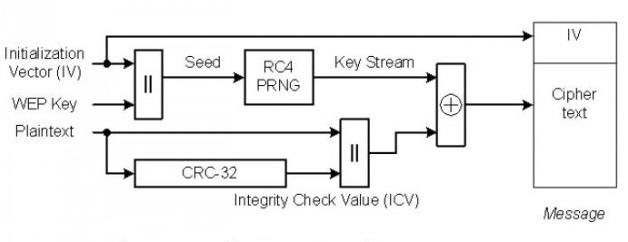
\includegraphics[height=2in]{WEPsummary}
\caption{Visual Summary of WEP}
\label{fig:WEPsummary}
\end{figure}

\subsection{The IV}
As mentioned above, the root key is attached to a variable IV of 24 bits before being used to initialize the stream cipher.  The IV changes for each packet, resulting in a different key stream for each encryption.  This should greatly diminish the significance (and the likelihood) of an attacker finding one key stream to almost nothing, as there supposedly would then be little chance of that IV ever being used again.

\subsection{RC4}
The RC4 stream cipher is used to produce the key stream, one byte at a time, based off an internal state.  This state consist of a permutation of the numbers 0-255 stored in an array S, and of two variables i and j such that $0\leq i,j\leq 255$.  The initial order of S is determined by the \textit{ RC4 Key Scheduling Algorithm} (RC4-KSA) as a function of the key (which is determined as the IV prepended to the  root key), and i and j are initially 0.  Bytes are produced to the key stream via the \textit{RC4 Pseudo Random Generator Algorithm} (RC4-PRGA).  Before each byte is produced to the key stream, this algorithm slightly reorders the elements of S, and updates the values of i and j.  The returned byte is (S[i]+S[j]) mod 256.
\begin{figure}[t]
\centering
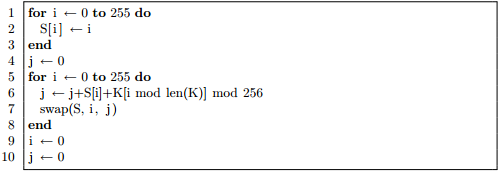
\includegraphics[height=1.5in]{RC4KSA}
\caption{RC4 Key Scheduling Algorithm}
\label{fig:rc4ksa}
\end{figure}
\begin{figure}[b]
\centering
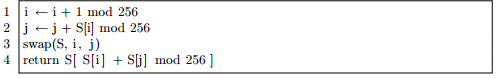
\includegraphics[height=.7in]{RC4PRGA}
\caption{RC4 Psuedo Random Generator Algorithm}
\label{fig:rc4prga}
\end{figure}

\subsection{CRC-32}
\label{sec:crc}
CRC-32 (for 32-bit Cyclic Redundancy Checksum) is an error-detecting function which serves to detect changes to data.  The function is essentially polynomial division, where the dividend is the payload and the divisor is a standard 33 bit number predetermined for its suitability in error correction.  The bits of the payload and the 33 bit number each function as the coefficients of their respective polynomial.  For example, the number 1011 represents the polynomial $1x^3+0x^2+1x+1$.  In bitwise division, this corresponds to cyclic XORing of bits, maintaining a property of linear mapping, where $CRC32(x\oplus y)=CRC32(x)\oplus CRC32(y)$.

\subsection{802.11 Wireless \& Authentication}
802.11 is a set of IEEE specifications for implementing Wireless Local Area Network (WLAN) communications.  By this standard, every network is identified by a name, called its ESSID.  This is typically a short string, such as \textit{PublicCafeWifi} or \textit{HotelNetwork}.  The IEEE's 802.11 defines two types of networks: the infrastructure network and the ad hoc network.  In an ad hoc network, stations communicate directly with each other, without any central component.  This is seldom used.  An infrastructure network uses a \textit{Basic Service Set} (BSS) as a base station to the others.  It is also denoted an \textit{Access Point} (AP) when it provides access to a local network.  Every AP is identified by a BSSID, its MAC address. Most AP’s broadcast their BSSID and ESSID in intervals of about .1 sec.  Clients who want to become members of the network have to associate with a point using a handshake.  Some network operators disable the broadcasting, thereby making their networks “hidden.”  In this case, the client must first send the ESSID of the network he wants to join.
\\\\
Authentication with the AP happens via the “handshake” mentioned above.  For a network configured to open system authentication (no password), all this requires is that the client send a request and the AP will respond with success.  With the Shared Key authentication configuration, the client first sends a request as before.  Now, however, the AP will send a random string of bytes as a challenge.  The client then needs to encrypt that string using the shared (root) key and send it back.  If the AP is able to decrypt it to the original string, then it knows that the client possesses the shared key and will reply with success.
\begin{figure} [h]
\centering
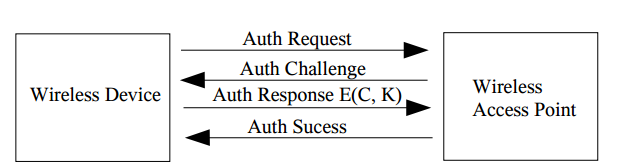
\includegraphics[height=1.5in]{Authentication}
\caption{Shared Key Authentication}
\label{fig:Authentication}
\end{figure}

\newpage
% 4th section
\section{Vulnerabilities and Exploitations}
\label{sec:vuln}
The RC4 stream cipher is not a reliable method of encryption, due both to its byte by byte method of encryption and its failure to sufficiently randomize the initial permutation of the array S.  By analyzing and/or manipulating multiple messages encrypted with the same key, attackers have found ways to recover the key stream and even the root key itself.  WEP specifies the use of a variable IV to prevent key stream reuse, and uses a 32 bit checksum to maintain data integrity.  Neither of these measures, however, as we shall show, are sufficient to stop or significantly slow down an attacker.  Following a description of the weaknesses of the IVs and CRC32, we will delve into an explanation of fake authentication - another necessary obstacle to overcome before many direct attacks on RC4 - and lastly we will explain some direct attacks themselves.

\subsection{Small IV space}
The IV used in WEP is 24 bits, so there are only $2^{24}<$ 17 million possible IVs.  On a network with moderate traffic, this space is exhausted in less than 5 hours, meaning that waiting for a key collision is at least very feasible for an attacker.  Using packet injection, he can dramatically increase the traffic so the time required may be even less.  The small IV space also makes a dictionary approach possible, requiring only 15-25 GB of storage to record all possible IV - key stream pairs for a given root key.

\subsection{CRC-32 Weakness}
A ciphertext $C$ consists of an encrypted payload $E$ followed by its encrypted checksum $CRC32(E)$.  By changing E in the desired way to E' and then changing the encrypted checksum to CRC32(E') we create a modified ciphertext C'.  The decryption of C' produces a payload P' (a modification of an original payload P) followed by a decryption of CRC32(E').  We will show that this equals CRC32(P'), signifying that the message will authenticate under these modifications.  As specified in section~\ref{sec:crc}, it is a linear function with the property $CRC32(x\oplus y)=CRC32(x)\oplus CRC32(y)$.  This property will be used in the following proof.
\\\\
Let $\Delta = E \oplus E'$.  That is, $\Delta$ represents the changes from $E$ to $E'$.  Then
\[CRC32(E) \oplus CRC32(E') = CRC32(E \oplus E') = CRC32(\Delta).\]
So $CRC32(\Delta)$ represents the changes from $CRC32(E)$ to $CRC32(E')$. Consequently
\[C \oplus C' = [E,CRC32(E)] \oplus [E',CRC32(E')] = [\Delta , CRC32(\Delta)]\]
From this, it follows that
\begin{align*}
C' &= C \oplus [\Delta , CRC32(\Delta)]\\
   &= RC4(IV,R_k)\oplus [P,CRC32(P)]\oplus [\Delta , CRC32(\Delta)]\\
   &= RC4(IV,R_k)\oplus [P\oplus \Delta, CRC32(P)\oplus CRC32(\Delta)]\\
   &= RC4(IV,R_k)\oplus [P', CRC32(P\oplus \Delta)]\\
   &= RC4(IV,R_k)\oplus [P', CRC32(P')]\\
\end{align*}
Thus we see that $C'$ is identical to a modified payload P' and its checksum encrypted with the same key stream as was used in the encyption of [P, CRC32(P)].
\\\\
It is worth noting that CRC was invented as an error-correcting mechanism, capable of detecting \textit{accidental} changes to data, and was never intended to prevent purposeful tampering.  Consequently, it should never have been relied on to detect or prevent intentional manipulation in a protocol such as WEP.

\subsection{Illicit Authentication and Packet Injection}
In order to inject packets and interact with the AP in other ways that may be required for an attack, an attacker must be authorized as a client.  Per the procedures outlined earlier in the report, this would normally require using the shared key to generate a key stream and encrypt the challenge text.  However, because both the challenge and its response are sent through the air in an authentication, an attacker can simply sniff a valid handshake and XOR the challenge with its response.  This will generate a key stream which he can then use to correctly encrypt the challenge text he receives upon requesting authentication for himself.  Keep in mind this is only a step in the hacking process, and not the goal itself.  At this point, an attacker only has permission to send traffic through and receive traffic from the AP, but because he does not have the key, he can neither encrypt traffic to send nor decrypt packets received.  However, that does not matter for packet injection, so the attacker will still gain leverage in the ability to create much more traffic on the network, thus generating more IV - ciphertext pairs for analysis, and leading to a shorter cracking time.
\\\\
Because some networks might see new authentications with relative infrequency, whether due to a low quantity of users or because most machines on them are perpetually connected, it would be desirable in many circumstances to have an alternative method of fake authentication.  There may be possibility in some cases of forcing another station to re-authenticate itself immediately, allowing for the attacker to sniff a challenge and its response without delay.  Spoofing the MAC of an already associated client would also allow access.  Lastly, an attacker might uncover a IV - key stream pair using fragmentation methods described in section~\ref{sec:frag} .

\subsection{Dictionary Attack}
A dictionary attack is accomplished by using weaknesses in the RC4 encryption to obtain key streams corresponding to known IVs when multiple packets encrypted with the same key are known. The table of these key stream - IV pairs is referred to as the dictionary. Using some of the initially developed attacks, this method requires up to two weeks of packet sniffing to find enough key collisions for every IV, although this can be sped up using packet injection to generate a higher volume of traffic. Regardless of the time taken to build a dictionary, this type of attack requires up to 25GB of memory, a decent yet feasible resource requirement. This attack does not yield the root key, but the attacker can still perform any desired function on the network.  Because the IV’s are broadcast with every packet, once a dictionary is complete the attacker can decrypt any packet that is broadcast. He can also encrypt packets to send while knowing the proper IV to send with them.

\subsection{Fragmentation Attack}
\label{sec:frag}
A fragmentation attack is based on the fact that we can deduce with excellent certitude the first seven bytes of a packet which contain the preamble of the ethernet frame.  The corresponding seven bytes of the key stream can be deciphered because if one knows a plaintext and the corresponding ciphertext, the section of the key stream used to encrypt the known parts can be determined. Using this section of the key stream, an ARP packet can be created that can be sent to the AP.  The AP will reply with a packet of which thirty-six bytes of key stream can be deduced. This process can be repeated again and again until 1500 bytes of key stream are captured. Once this is achieved, any packet that is desired can be sent on the network because data is sent in packets of not more than 1500 bytes. The network is already partially compromised at this point because an attacker can send any packet they want to through the router. This attack is commonly used to execute a fake authentication without needing to wait for a valid handshake to be sniffed.

\subsection{Statistical Attack}
While the dictionary attack only results in a huge table after a long period of sniffing, other probability-based attacks can result in direct knowledge of the root key in far less time. A statistical attack is a way of generating the root key by using “weak initialization vectors.” This method of attack uses the fact that for certain IVs there are sections of the key stream that correspond by specific functions of the IV to specific parts of the root key. For a single given packet this is not even close to 100\% accurate. In fact the accuracy for a specific initialization vector is, as Rafik Chaabouni says, between 5\% and 13\%. This is of course much higher than a random guess and this process is repeated with different IVs in conjunction with the birthday paradox to further improve the chances to near 100\%. Once the first byte of the root key is defined, the next byte becomes more predictable. This allows guesses to be strung together efficiently and significantly decreases the brute force search space. The majority of the implementations currently in use are of this type, using probability to reach a guess close to the root key and using brute force to find the less definite bits. This is in fact the approach used in the attack we will implement using aircrack-ng.



\newpage
% 5th section
\section{Implementation}
\label{sec:implmnt}
After setting up a router with WEP encryption, we were able to successfully recover a root key using the attacks of fake authentication via fragmentation, packet injection, and statistical analysis as implemented in the aircrack-ng suite.
\\\\
A few parameters had to be gathered before running the attack.
MAC of attacker's computer (us): 00:e0:4c:00:f0:65\\
BSSID (MAC of access point): 64:66:B3:2E:CE:EE\\
ESSID (Wireless network name): ByteMe\\
Access point channel: 4\\
Wireless interface: wlan0\\
\\
1. Find the MAC of the AP using the command:\\
\begin{center}
\texttt{iwlist wlan0 scan}
\end{center}

\begin{figure}[h]
\centering
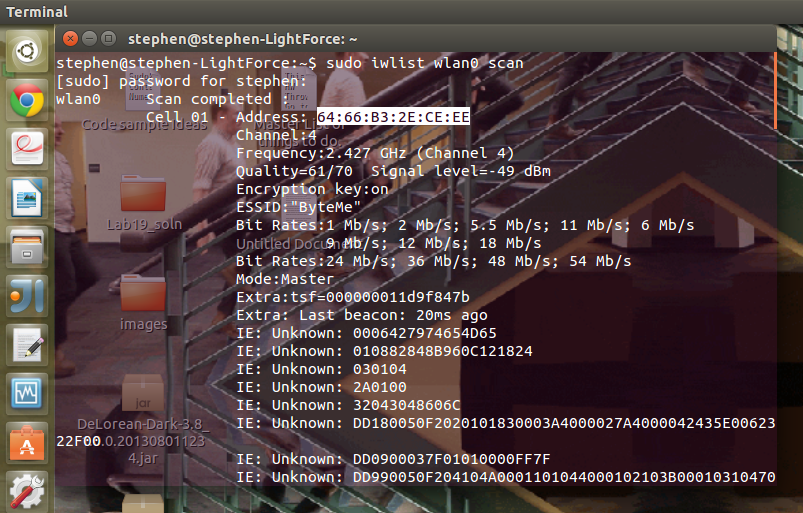
\includegraphics[height=3in]{findMAC'sAP}
\caption{Scanning for the AP to find its MAC}
\label{fig:MACAP}
\end{figure}

2. Test packet injection using the command
\begin{center}
\texttt{aireplay-ng -9 -ByteMe -a 64:66:B3:2E:CE:EE wlan0}
\end{center}
where \texttt{-9} specifies an injection test.  The 100\% at the bottom of the output and the message "\texttt{Injection is Working!}"designate success (See Figure~\ref{fig:injectest}).
\\\\\\\\\\

\begin{figure} [h]
\centering
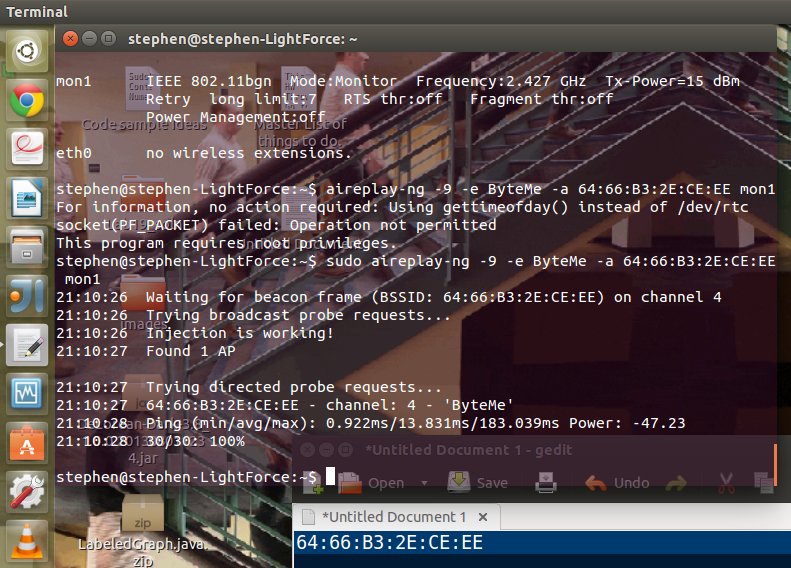
\includegraphics[height=3in]{InjectionTest}
\caption{Testing Packet Injection}
\label{fig:injectest}
\end{figure}

3. Open another terminal (on the right in Figure~\ref{fig:ivcapt}) and capture IVs using the command
\begin{center}
\texttt{airodump-ng -c 4 --bssid 64:66:B3:2E:CE:EE -w output wlan0}
\end{center}
where \texttt{4} is the AP channel and \texttt{output} is the name of the file which will record the IVs.
\\\\\\
\begin{figure} [h]
\centering
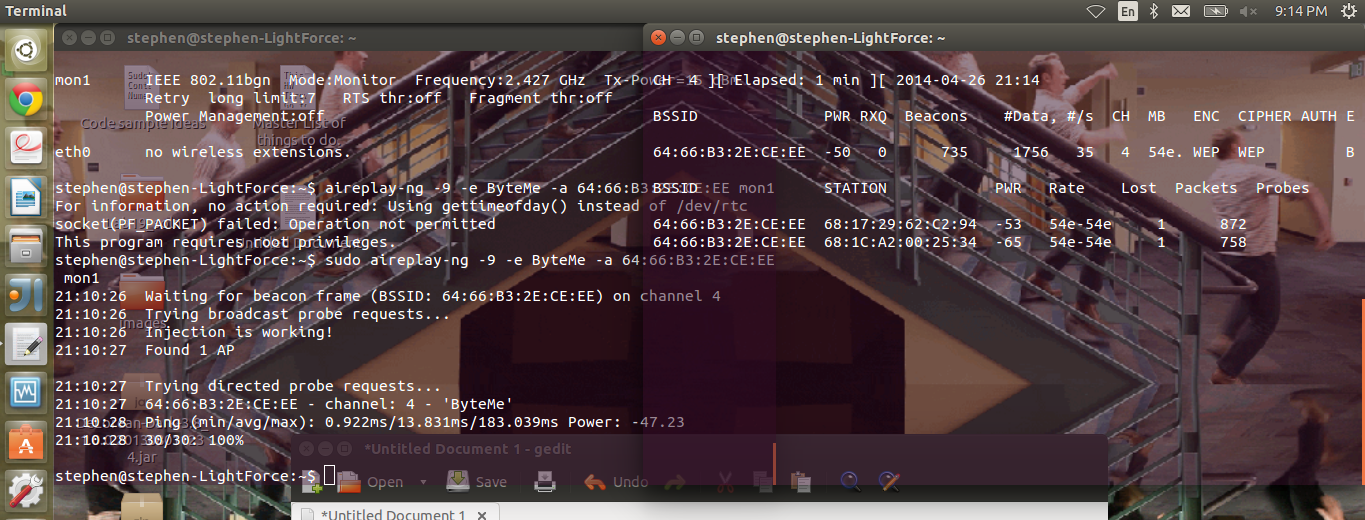
\includegraphics[height=2.8in]{IVCapture}
\caption{Capturing IVs}
\label{fig:ivcapt}
\end{figure}

4. Perform fake authentication with the command
\begin{center}
\texttt{aireplay-ng -1 0 -e ByteMe -a \newline 64:66:B3:2E:CE:EE -h 00:e0:4c:00:f0:65 wlan0}
\end{center}
where \texttt{-1} specifies fake authentication and \texttt{0} is the reassociation time in seconds.  This uses the fragmentation attack discussed in section \ref{sec:frag}.
\\\\
\begin{figure} [h]
\centering
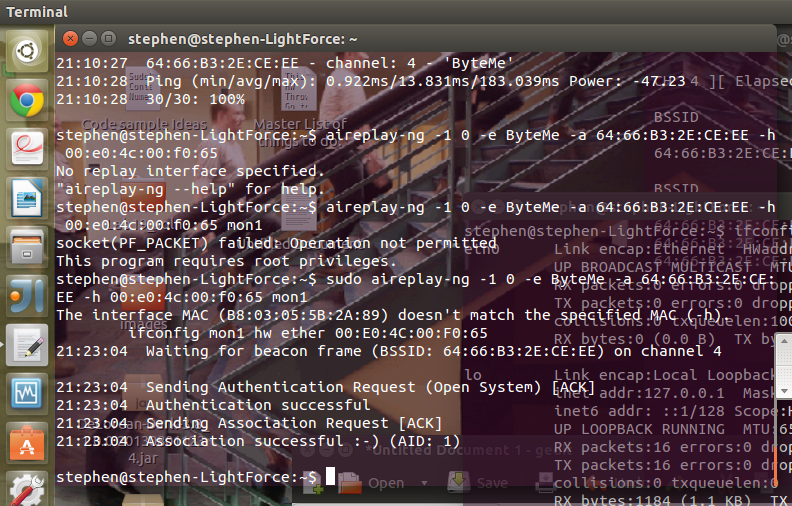
\includegraphics[height=3in]{FakeAuthentication}
\caption{Successful Fake Authentication}
\label{fig:fakeauth}
\end{figure}

5. Peform packet reinjection with the command
\begin{center}
\texttt{aireplay-ng -3 -b 00:14:6C:7E:40:80 -h 00:0F:B5:88:AC:82 wlan0}
\end{center}
This command is constructed to listen for and reinject ARP requests because the AP will normally rebroadcast them immediately, thereby generating more IVs.  This creation of more traffic to speed up the attack in the next step is the goal here.  This step can be seen running in the background on the left in Figure~\ref{fig:keyfnd}.
\\\\\\\\\\\\\\\\\\\\\\\\

6. Run the statistical analysis attack with the command
\begin{center}
\texttt{aircrack-ng -b 00:14:6C:7E:40:80 output.cap}
\end{center}
where \texttt{output.cap} is the file where we stored captured IVs.  This attack failed for us a few times before it gathered enough IV to correctly discover the root key.

\begin{figure} [h]
\centering
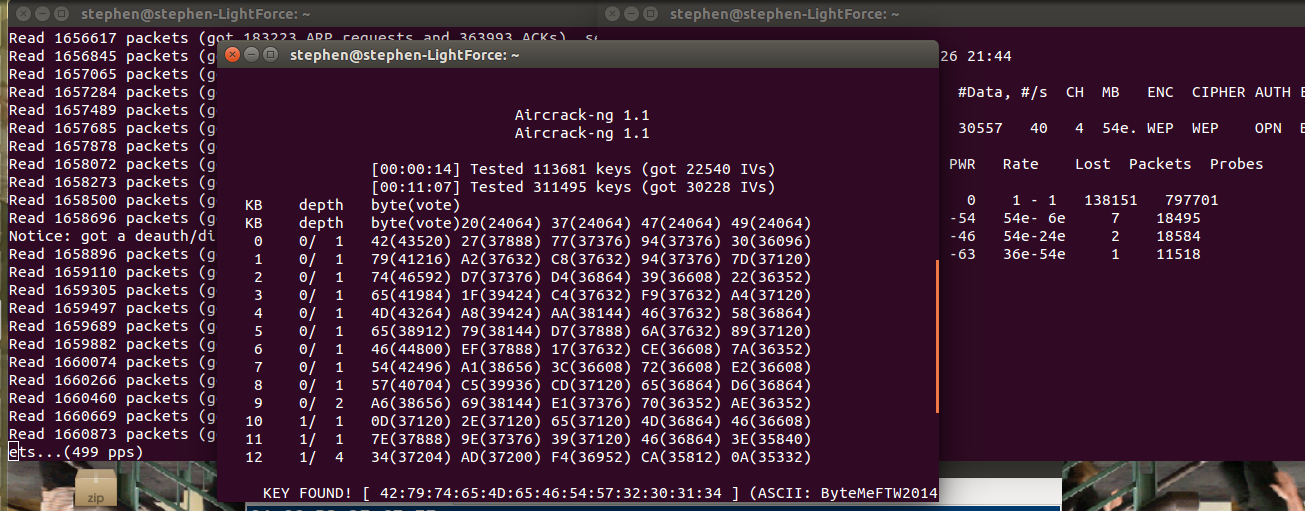
\includegraphics[height=3in]{KeyFound}
\caption{Aircrack found the Key!}
\label{fig:keyfnd}
\end{figure}

Upon the attack being successful, we are told that the key is \texttt{ByteMeFTW2014}.

\newpage
\section{Defenses}
\label{sec:def}
The best defense against the weaknesses of WEP is to use a secure Wi-Fi encryption system instead of WEP.  The current secure standard is WPA2, and as WEP has been known to be insecure since 2001 and officially outdated since 2004, no one should still be using it.
\\\\
There are, nonetheless, a few ways the WEP system might have been made at least slightly more secure without completely changing it to a new protocol.  Although the RC4 stream cipher is the heart of WEP's failure, we will refrain from speaking of improvements on it in considering improvements to WEP, as such considerations would more properly fall under the category of implementation of a distinct protocol.
\\\\
The small IV space, 'weak' IVs, and the existence of predictable key streams are all issues related to the IV.  Simply increasing the IV to 32 bits would multiply the time taken to exhaust all possibilities by $2^8=256$, thus reducing the likelihood of a key collision drastically and transforming an attack of an hour or two into one which would takes days or months.  The RC4-KSA algorithm allows for a key of up to 256 bits in creating its internal state, so the key could be divided into a 64 bit root key and a 64 bit IV.  This would extended the IV space to $2^{64}=1.845\times 10^{19}$, making a wait for key collision almost hopeless.  To make the key stream less predictable, a preset initial portion of the key stream, which is usually the most predictable, could be discarded.  Alternatively, or in addition, the IV could be appended to the root key rather than prepended.  Some attacks are at least partially based on some of the first bytes of the internal array being determined from the known IV, so swapping the IV and root key before key stream formation would result in these beginning bits being less determinable from the known IV.  Some particulars IVs are also known to be weak due to failure to significantly randomize the bit stream more than others.  Disallowing the use of these IVs could potentially make the system more secure, though depending on the number of such IVs, doing this might also significantly decrease the key space, making the system weaker in that respect.
\\\\
To prevent manipulation of packets, a secure hash algorithm might have been used in place of the CRC32.
\\\\
Improvements similar to some of the above suggestions have been implemented.  However, because the weakness lies primarily in the RC4 encryption, all the modified versions that were ever used much at all have successfully been hacked, though it \textit{might} take slightly longer for some of them.  This demonstrates pretty clearly that the time has come, and had indeed come long ago, for the replacement of WEP with a completely new protocol.  Using the current standard of WPA2 is indeed the best and possibly the only real defense.

\newpage
\section{Synthesis}
\label{sec:synth}
Due to the increased prevalence of Wi-Fi usage, the need to prevent unauthorized access is more important than ever.  With no encryption, anyone within range of a Wi-Fi network could access the internet (and potentially user files and servers, depending on shared resource settings), thereby slowing down access for the intended users.  No encryption would also allow an attacker within range to “sniff” packets transmitted through the air and view them, allowing him to see what other users are sending and receiving, thus violating their privacy.  This is a serious concern in many cases, so the need for strong link layer security is important.  Its importance will only increase, as every indicator points to wireless communication being the future for home and office networks.  WEP was an attempt to achieve this security, and one which failed miserably.  Because an attacker can crack the key with relative ease and can modify a message in transit without detection, WEP is a failure in both confidentiality and integrity.  Most of the world has moved on to WPA2, but the significance of this problem designates a need for every last straggler to do so.

\newpage
% Bibliography (simple)
% For more complex / reusable bibliography, search online for 'Bibtex' .
% Bibtex-format citations can be exported from OneNote, etc. and stored
% in .bib files to be included in .tex files.  The below syntax is for short,
% simple bibliographies.
\begin{thebibliography}{1}
\bibitem{} Borisov, Nikita, Ian Goldberg, and David Wagner. "(in)Security of the WEP Algorithm." \textit{berkley.edu}. Berkley, 2001. Web. 2 May 2014.
\bibitem{} Bittau, Andrea, Mark Handely, and Joshua Lackey. "The Final Nail in WEP's Coffin." \textit{www.tapir.cs.} N.p., 2006. Web. 2 May 2014.
\bibitem{} DarkAudax. "Tutorial: Simple WEP Crack." \textit{www.aircrack-ng.org}. Aircrack, 2010. Web. 02 May 2014.
\bibitem{} Tews, Erik. Attacks on the WEP Protocol. \textit{www.cs.rit.edu/}. TU Darmstadt, 2007. Web. 2 May 2014.
\bibitem{} Borisov, Nikita, Ian Goldberg, and David Wagner. "Intercepting Mobile Communications\:
The Insecurity of 802.11" \textit{berkley.edu}. Berkley, 2001. Web. 2 May 2014.

\end{thebibliography}
\end{document}



